\documentclass{article}

\usepackage[utf8]{inputenc}
\usepackage[T1]{fontenc}
\usepackage[norsk,english]{babel}   %Norsk først så engelsk, så engelsk blir prioritert
\usepackage{graphicx}
\usepackage{amsmath}        %For å kunne skrive matte
\usepackage{listings}       %For å kunne skrive inn kode med fin formatering
\usepackage{multicol}       %Importerer pakken for multikolonner til teksten
\usepackage[margin=2.54cm]{geometry}    %Definerer hva bredden til teksten er
\usepackage{wrapfig}    %Importerer pakken for å ha bildene i teksten
\usepackage[font = small]{caption}

%Definerer hyperlinker og dens farger
\usepackage{hyperref}
\hypersetup{
    colorlinks,
    citecolor=blue,
    filecolor=black,
    linkcolor=blue,
    urlcolor=blue
}

%-----------------------------------

%Definerer farger til kodeeksemplene i PDF-en
\usepackage{color}

\definecolor{codegreen}{rgb}{0,0.6,0}
\definecolor{codegray}{rgb}{0.5,0.5,0.5}
\definecolor{codepurple}{rgb}{0.58,0,0.82}
\definecolor{backcolour}{rgb}{0.95,0.95,0.92}

\lstdefinestyle{mystyle}{
    backgroundcolor=\color{backcolour},
    commentstyle=\color{codegreen},
    keywordstyle=\color{magenta},
    numberstyle=\tiny\color{codegray},
    stringstyle=\color{codepurple},
    basicstyle=\footnotesize,
    breakatwhitespace=false,
    breaklines=true,
    captionpos=b,
    keepspaces=true,
    numbers=left,
    numbersep=5pt,
    showspaces=false,
    showstringspaces=false,
    showtabs=false,
    tabsize=2
}

\lstset{style=mystyle}

%------------------------------------

\setlength{\parindent}{0pt} %Ingen indent automatisk for nye linjer
%\setlength{\columnsep}{2mm} %Column separation - til multicolumn

%\setlength{\arrayrulewidth}{1mm}   %Hvilken tykkelse tabellene skal ha
\setlength{\tabcolsep}{2mm}     %Lengden mellom hver kolonne
\renewcommand{\arraystretch}{1.5}   %Hvor stor avstand det skal være mellom radene

\iffalse    %midlertidig endre bredden på teksten
If you want to change this temporarily, you can write:
\savegeometry{mydefaultgeometry}
\newgeometry{margin=3in}
And then later you can call:
\loadgeometry{mydefaultgeometry}
\fi

%for å fjerne overskriften "refrences" som kommer automatisk når man bruker bibtex
\usepackage{etoolbox}
\patchcmd{\thebibliography}{\section*{\refname}}{}{}{}

%----------------------------------------------------------------------------------------

\begin{document}

\addtocounter{page}{0}

\title{Project 4 \\
      \large For the course FYS3150}
\date{\today \\
    \vspace{1mm}
    \large Week 43 - ?}

\author{Erik Grammeltvedt, Erlend Tiberg North and Alexandra Jahr Kolstad}

\maketitle

%\newpage

%------------Her starter skrivingen-----------------------------------------

%\begin{multicols}{2}

\textbf{TING Å GJØRE}
\begin{itemize}
  \item a) ferdig
  \item b) code is ran, discuss results
  \item c) code is ran, discuss results (see RESULTS.txt)
  \item d) code is ran, see probability-distribution.py (input energy/L20.....txt)
  \item e) currently running, need plotting-program and timing analysis!
  \item f) TRENGER ALT
\end{itemize}

\iffalse
TEXTCHAT:


\fi


%-------------------- Abstract -------------------------------
\vspace{1cm}


\begin{center}

{\Large\textbf{Abstract}} \label{sec:Abstract}

\end{center}

In this numerical project we have simulated some solid-state properties using the two-dimensional Ising model. The system was comprised of flippings spins, and they simulated energies, heat capacity, magnetization and susceptibility.
The results were FORTELL NOE OM RESULTATENE

\newpage

%------------------- Table of contents -----------------------

\vspace{1cm}

\tableofcontents

\vspace{1cm}

%-------------------- Introduction ------------------------------
\vspace{1cm}

\section{Introduction} \label{sec:Introduction}

The simulation consisted of a 2-dimensional lattice with spins pointing up or down. They

%-------------------- Theory ------------------------------------
\vspace{1cm}

\section{Theory} \label{sec:Theory}

\subsection{Analytical solution for \texorpdfstring{ $2 \times 2$ }{text} lattice}

The energies in this lattice is given by the set $E_i = \{- 8 J, -4J, 0 , 4J, 8J \}$.

Tallene her er ikke oppdaterte, spesielt for energiene

$$ \langle E \rangle = - 7.98393 $$
$$ \langle E^2 \rangle = 15.96786 $$
$$ C_V = (15.96 - (-7.98)^2) = -47.77528 \hspace{1cm} ???????? $$

$$ \langle M \rangle = 0 \hspace{1cm} ???????????????? $$
$$ \langle M^2 \rangle = 15.97322$$
$$ \chi = (15.97322 - (0)^2) = 15.97322 $$


\subsubsection{Partition function}

The partition function is given by the equation below.

\begin{equation} \label{eq:partitionfunction}
    Z = \sum_{i=1} ^{M} e^{- \beta E_i}
\end{equation} \\

The sum runs from 1 to $M$, which is 16 because of the $ 2 \times 2 $ lattice. To calculate the partition function we need to know that

\begin{equation*}
    2 \cosh (x) = e^x + e^{-x}
\end{equation*} \\

Calculating the partition function.

\begin{align*}
  Z &= \sum_{i=1} ^{M} e^{- \beta E_i} = \sum_{i=1} ^{16} e^{- \beta E_i} \\
  &= 1 \cdot e^{- \beta (-8J)} + 4 \cdot e^{- \beta (0J)} + 2 \cdot e^{- \beta (8J)} + 4 \cdot e^{- \beta (0J)}
  + 4 \cdot e^{- \beta (0J)} + 1 \cdot e^{- \beta (-8J)} \\
  &= e^{8 \beta J} + 4 + 2 \cdot e^{-8 \beta J} + 4 + 4 + e^{8 \beta J} \\
  &= 2 e^{8 \beta J } + 2 e^{-8 \beta J} + 12 \\
  &= 2 \left( e^{8 \beta J} + e^{- 8 \beta J} \right) + 12 \\
  &= 2 \left( 2 \cosh(8 \beta J) \right) + 12 \\
  &= 4 \cosh(8 \beta J) + 12
\end{align*} \\

The partition function for this system is therefore given by $Z = 4 \cosh(8 \beta J) + 12$.

\subsubsection{Energy and mean magnetization}

The expectation value of the energy is

\begin{equation}    \label{eq:expectationenergy}
    \langle E \rangle = \frac{1}{Z} \sum _{i=1} ^M E_i e^{- \beta E_i} \\
\end{equation} \\

In addition we need to know that

\begin{equation*}
    2 \sinh (x) = e^x - e^{-x}
\end{equation*} \\

The expectation value of the energy is

\begin{align*}
  \langle E \rangle &= \frac{1}{Z} \sum _{i=1} ^M E_i e^{- \beta E_i} \\
  &= \frac{1}{Z} \left[ 1 \cdot (-8J) e^{- \beta (-8J)} + 4 \cdot 0 + 2 \cdot (8J) e^{- \beta (8J)} + 4 \cdot 0 + 1 \cdot (-8J) e^{- \beta (-8J)} \right] \\
  &= \frac{1}{Z} \left[ - 8J e^{\beta 8J} + 2 \cdot 8J e^{- \beta 8J} - 8J e^{ \beta 8J} \right] \\
  &= \frac{2}{Z} \left[ - 8J e^{\beta 8 J} + 8 J e^{- \beta 8 J} \right] \\
  &= - \frac{16 J}{Z} \left( e^{8 \beta J} - e^{- 8 \beta J} \right) \\
  &= - \frac{16 J}{Z} (2 \sinh(8 \beta J) ) \\
  &= - \frac{32 J}{Z} \sinh(8 \beta J)
\end{align*} \\

The expectation value of the mean magnetization is

\begin{equation}    \label{eq:meanmagnetization}
    \langle M \rangle = \frac{1}{Z} \sum _{i=1} ^M M_i e^{- \beta E_i} \\
\end{equation} \\

For this system it is

\begin{align*}
  \langle M \rangle &= \frac{1}{Z} \sum _{i=1} ^M M_i e^{- \beta E_i} \\
  &= \frac{1}{Z} \left[1 \cdot 4 e^{- \beta (-8J)} + 4 \cdot 2 e^{- \beta (0J)} + 2 \cdot 0 + 4 \cdot 0 + 4 \cdot (-2) e^{- \beta (0J)} + 1 \cdot (-4) e^{- \beta (-8J)} \right] \\
  &= \frac{1}{Z} \left[ 4 e^{\beta 8J} + 8 - 8 - 4 e^{ \beta 8J} \right] \\
  &= \frac{1}{Z} \cdot 0 \\
  &= 0
\end{align*} \\


\subsubsection{Specific heat}

The specific heat is given by the equation

\begin{equation}    \label{eq:specificheat}
    C_V = \frac{1}{k_B T^2} \left( \langle E^2 \rangle - \langle E \rangle ^2 \right)
\end{equation} \\

Therefore the expectation value of the energy squared has to be calculated.

\begin{align*}
  \langle E^2 \rangle &= \frac{1}{Z} \sum _{i=1} ^M E_i^2 e^{- \beta E_i} \\
  &= \frac{1}{Z} \left[ 1 \cdot (-8J)^2 e^{- \beta (-8J)} + 4 \cdot 0 + 2 \cdot (8J)^2 e^{- \beta (8J)} + 4 \cdot 0 + 1 \cdot (-8J)^2 e^{- \beta (-8J)} \right] \\
  &= \frac{1}{Z} \left[ 64 J^2 e^{\beta 8J} + 2 \cdot 64 J^2 e^{- \beta 8J} + 64 J^2 e^{ \beta 8J} \right] \\
  &= \frac{2 \cdot 64 J^2}{Z} \left[ e^{\beta 8 J} + e^{- \beta 8 J} \right] \\
  &= \frac{128 J^2}{Z} (2 \cosh(8 \beta J) ) \\
  &= \frac{256 J^2}{Z} \cosh(8 \beta J)
\end{align*} \\

Now the specific heat can be calculated.

\begin{align*}
    C_V = \frac{1}{k_B T^2} \left( \langle E^2 \rangle - \langle E \rangle ^2 \right)
    &= \frac{1}{k_B T^2} \left( \frac{256 J^2}{Z} \cosh (8 \beta J) - \left( - \frac{32 J}{Z} \sinh(8 \beta J ) \right) ^2 \right)
\end{align*} \\


\subsubsection{Susceptibility}

The susceptibility is given by

\begin{equation}    \label{eq:susceptibility}
    \chi = \frac{1}{k_B T} \left( \langle M^2 \rangle - \langle M \rangle ^2 \right)
\end{equation} \\

The expectation value of the mean magnetization squared therefore has to be calculated.

\begin{align*}
  \langle M^2 \rangle &= \frac{1}{Z} \sum _{i=1} ^M M_i^2 e^{- \beta E_i} \\
  &= \frac{1}{Z} \left[1 \cdot 4^2 e^{- \beta (-8J)} + 4 \cdot 2^2 e^{- \beta (0J)} + 2 \cdot 0 + 4 \cdot 0 + 4 \cdot (-2)^2 e^{- \beta (0J)} + 1 \cdot (-4)^2 e^{- \beta (-8J)} \right] \\
  &= \frac{1}{Z} \left[ 16 e^{\beta 8J} + 16 + 16 + 16 e^{ \beta 8J} \right] \\
  &= \frac{1}{Z} \left[ 2 e^{8 \beta J} + 2 \right] \\
  &= \frac{32}{Z} \left( e^{8 \beta J} + 1 \right) \\
\end{align*}

Now calculating the susceptibility of the system.

\begin{align*}
    \chi &= \frac{1}{k_B T} \left( \langle M^2 \rangle - \langle M \rangle ^2 \right) \\
    &= \frac{1}{k_B T} \left[ \frac{32}{Z} \left( e^{8 \beta J} + 1 \right) - 0^2 \right] \\
    &= \frac{1}{k_B T} \frac{32}{Z} \left( e^{8 \beta J} + 1 \right) \\
\end{align*}



ERIK



%--------------------- Method ------------------------------------
\vspace{1cm}

\section{Method} \label{sec:Method}

ERIK

%--------------------- Results ----------------------------------
\vspace{1cm}

\section{Results} \label{sec:Results}

  \texttt{.txt}-files for all the raw data generated by the projects are up on our \href{https://github.com/Erikbgram/Fys3150}{GitHub}. \\

\subsection{2x2-lattice}

When comparing the analytical results for the 2x2-lattice to the numerical simulation we found the following. See Table (\ref{tab:analytical}).

  \begin{table}[ht]
    \centering
    \caption{2x2 - Analytical vs numerical values (output/L2\_n1000\_T1.0\_ord0.txt)}
    \vspace{2mm}
    \label{tab:analytical}
    \begin{tabular}{|c|c|c|}
        \hline
         & Analytical & numerical at T=1.0\\
        \hline \hline
        <E> & ALEXANDRA & -1.998 \\
        Cv & ALEXANDRA & 0.015984 \\
        $\chi$ & ALEXANDRA & 0.000999 \\
        <|M|> & ALEXANDRA & 0.9995 \\
        \hline
    \end{tabular} \\
    \hspace{0pt}\\
  \end{table}

Running the 2x2-simulation the following data arised. See figures (\ref{fig:energy_L2_n1000_T1.0_ord0}), (\ref{fig:energy_L2_n1000_T2.4_ord0}).

\begin{figure}[ht]
    \centering
    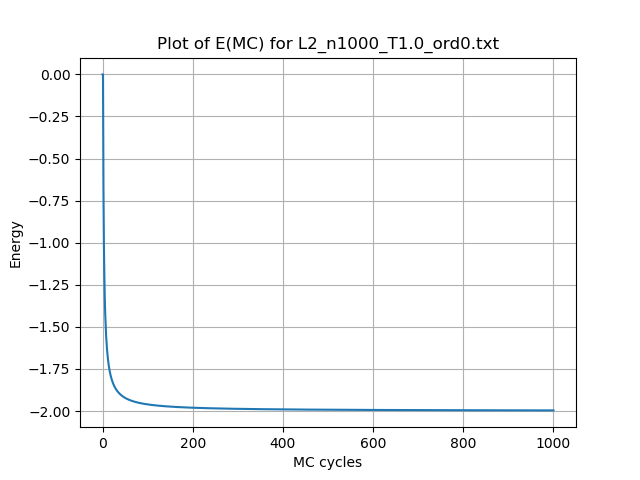
\includegraphics[width = 11cm]{img/energy_L2_n1000_T10_ord0.png}
    \caption{Energy-plot as function of MC-cycles. 2x2, MC1000, T=1.0, unordered spin}
    \label{fig:energy_L2_n1000_T1.0_ord0}
  \end{figure}

\begin{figure}[ht]
    \centering
    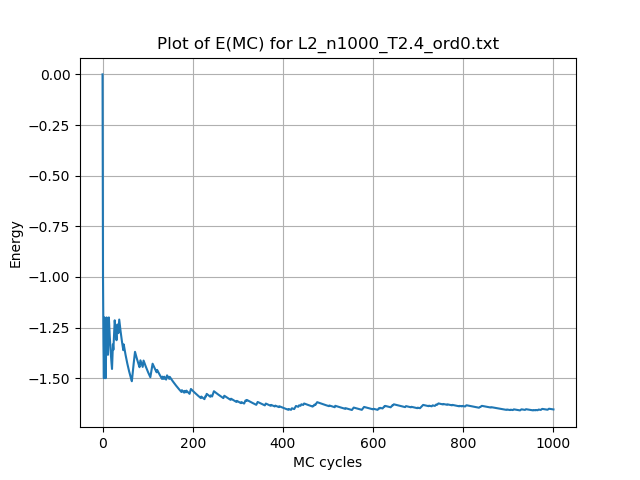
\includegraphics[width = 11cm]{img/energy_L2_n1000_T24_ord0.png}
    \caption{Energy-plot as function of MC-cycles. 2x2, MC1000, T=2.4, unordered spin}
    \label{fig:energy_L2_n1000_T2.4_ord0}
  \end{figure}

\begin{figure}[ht]
    \centering
    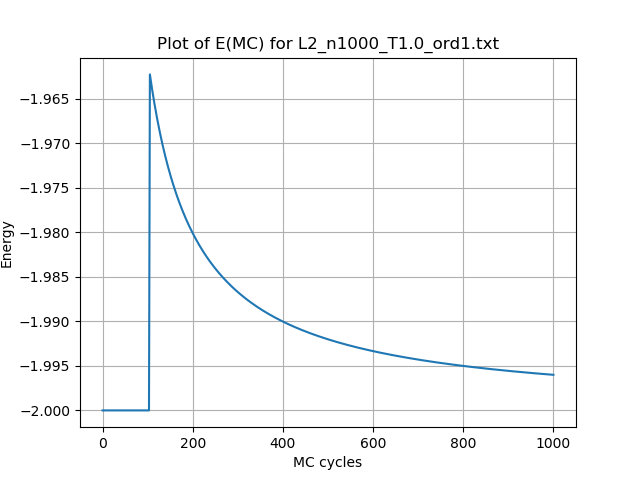
\includegraphics[width = 11cm]{img/energy_L2_n1000_T10_ord1.png}
    \caption{Energy-plot as function of MC-cycles. 2x2, MC1000, T=1.0, ordered spin}
    \label{fig:energy_L2_n1000_T1.0_ord1}
  \end{figure}

\begin{figure}[ht]
    \centering
    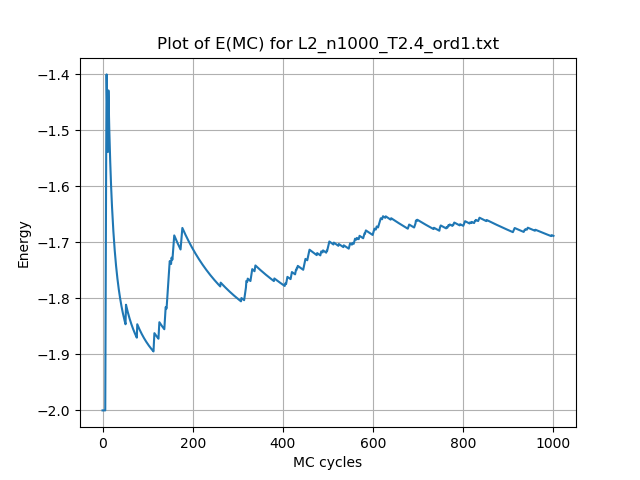
\includegraphics[width = 11cm]{img/energy_L2_n1000_T24_ord1.png}
    \caption{Energy-plot as function of MC-cycles. 2x2, MC1000, T=2.4, ordered spin}
    \label{fig:energy_L2_n1000_T2.4_ord1}
  \end{figure}

\subsection{20x20-lattice}

\subsubsection{Probability distributions}

\begin{figure}[ht]
    \centering
    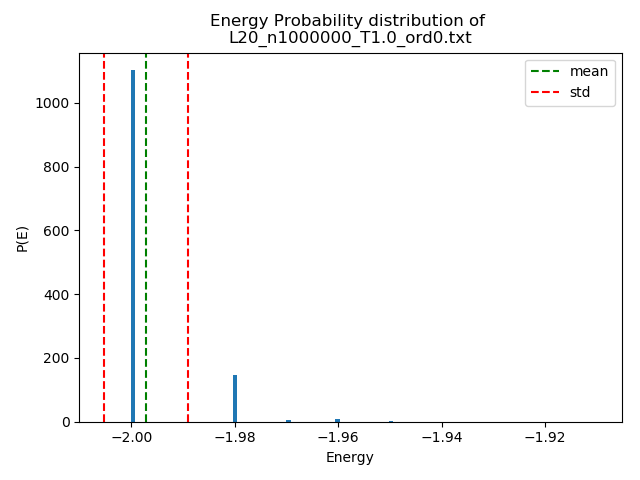
\includegraphics[width = 11cm]{img/energyhistogram_L20_n1000000_T10_ord0.png}
    \caption{Probability Distribution}
    \label{fig:prob-lowT-ord0}
  \end{figure}

\begin{figure}[ht]
    \centering
    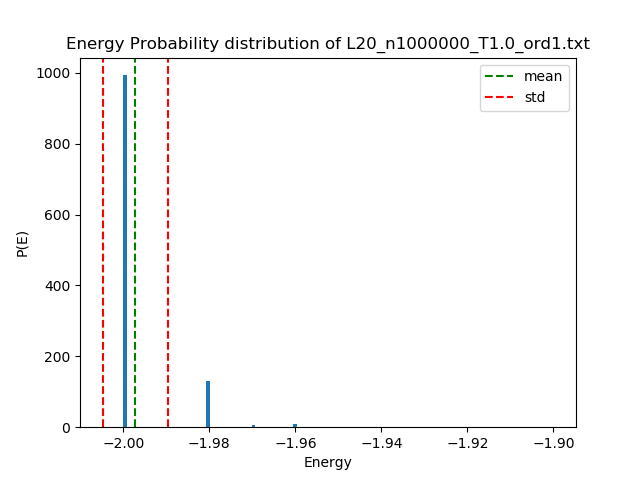
\includegraphics[width = 11cm]{img/energyhistogram_L20_n1000000_T10_ord1.png}
    \caption{Probability Distribution}
    \label{fig:prob-lowT-ord1}
  \end{figure}

\begin{figure}[ht]
    \centering
    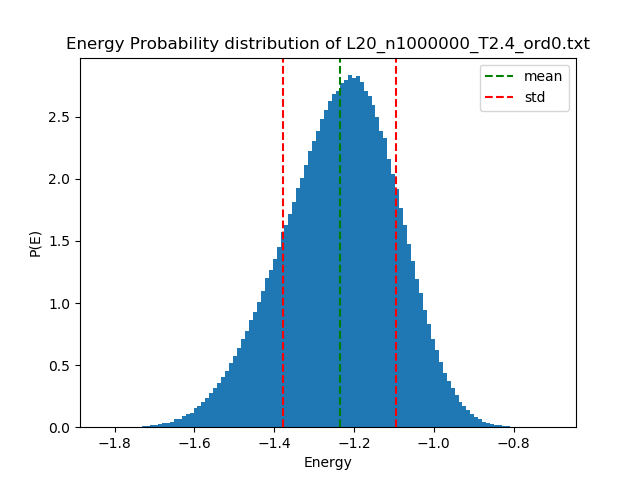
\includegraphics[width = 11cm]{img/energyhistogram_L20_n1000000_T24_ord0.png}
    \caption{Probability Distribution}
    \label{fig:prob-highT-ord0}
  \end{figure}

\begin{figure}[ht]
    \centering
    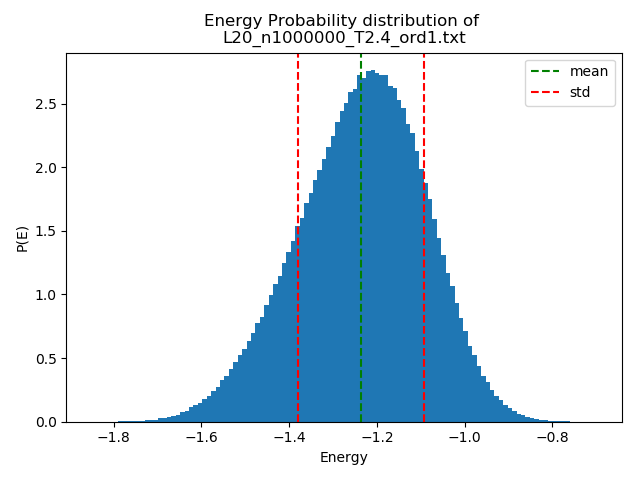
\includegraphics[width = 11cm]{img/energyhistogram_L20_n1000000_T24_ord1.png}
    \caption{Probability Distribution}
    \label{fig:prob-highT-ord1}
  \end{figure}

\subsection{Critical Temperature}

  \begin{table}[ht]
    \centering
    \caption{Critical temperature for simulations}
    \vspace{2mm}
    \label{tab:analytical}
    \begin{tabular}{|c|c|}
        \hline
         L & $T_c$\\
        \hline \hline
        40 & VALUE \\
        60 & VALUE \\
        80 & VALUE \\
        100 & VALUE \\
        \hline
    \end{tabular} \\
    \hspace{0pt}\\
  \end{table}

%--------------- Discussion ---------------------------------------
\vspace{1cm}

\clearpage
\newpage

\section{Discussion} \label{sec:Discussion}

Comparing the 2x2-lattice's numerical values with the analytical ones we see there is a major discrepancy. See table (\ref{tab:analytical}). This is quite unnerving. However, after many hours of debugging and re-checking analytical expressions, no reason was found, and as such the results have been left like that. The reason for this error could be from numerical errors, truncation errors hidden somewhere, faulty expressions or other similar explanations.

For 4c) see RESULTS.txt

ERIK


For 4d)

ERIK SE PÅ VARIANSEN

For 4e) ALEXANDRA

For 4f) ERIK


%---------------Conclusion and perspective---------------------------
\vspace{1cm}

\section{Conclusion and perspective} \label{sec:Conclusion}



%--------------Appendix---------------------------------------------
\vspace{1cm}

\section{Appendix} \label{sec:Appendix}

\subsection{Extracting the critical temperature}

In order to find the critical temperature we will use \cite{task}'s Eq. (3). It is shown below:
$$T_c(L)-T_c(L=\infty)=aL^{-1/\nu}$$
where $\nu=1$. This gives
$$T_c(L)-T_c(L=\infty)=\frac{a}{L}$$
In order to find $a$ we subtract the equation with different $L$-values.
$$T_c(L_{100})-T_c(L=\infty)=\frac{a}{L_{100}}$$
$$T_c(L_{80})-T_c(L=\infty)=\frac{a}{L_{80}}$$
Subtracting gives
$$T_c(L_{100})-T_c(L_{80})=\frac{a}{L_{100}-L_{80}}$$
$$(T_c(L_{100})-T_c(L_{80}))\cdot(L_{100}-L_{80})=a$$ \label{eq:finding-a}

%\clearpage

%----------------References----------------------------------------

\vspace{1cm}

\section{References} \label{sec:References}

\begin{thebibliography}{}

\bibitem{task}
Morten H. Jensen (2019), \href{https://github.com/CompPhysics/ComputationalPhysics/blob/master/doc/Projects/2019/Project4/pdf/Project4.pdf}{Project 4}, Departement of Physics, University of Oslo, Norway

\bibitem{github}
Erik B. Grammeltvedt, Alexandra Jahr Kolstad, Erlend T. North (2019), \href{https://github.com/Erikbgram/Fys3150}{GitHub}, Students of Departement of Physics, University of Oslo, Norway

\bibitem{lecture_slides}
Morten H. Jensen (2015), \href{https://github.com/CompPhysics/ComputationalPhysics/blob/master/doc/Lectures/lectures2015.pdf}{Lecture slides for FYS3150}, Department of Physics, University of Oslo, Norway

\bibitem{onsager}
Onsager (1944), \href{https://journals.aps.org/pr/abstract/10.1103/PhysRev.65.117}{"A Two-Dimensional Model with an Order-Disorder Transition"}, American Physical Society


\end{thebibliography}


%----------------Slutten av dokumentet---------------------------------------


%\end{multicols}

\end{document}
